\documentclass{article}
\usepackage[utf8]{inputenc}
\usepackage{textcomp}
\usepackage{version}
\usepackage{amsmath}
\usepackage{graphicx}
\usepackage[textwidth=8em,textsize=small]{todonotes}

\title{Analysis and visualization of the Heating Degree Days in the Benelux states}
\author{László Kiss \\ Senior Data Scientist, \\ ETH, Ericsson Hungary }
\date{March 2019}

\begin{document}

\maketitle

\section*{Abstract}
\paragraph{}Heating Degree Days is a technical measurement for calculating the energy demand to heat a buildings. Space heating is responsible for a large fraction of energy use. Heating Degree Days is a proxy for energy demand to heat a home or a business. This technical number derived from measurement of outside air temperature. However, it is also depend on a large number of other factors, in particular building design, energy prices, income levels and behavioural aspects. Space heating is responsible for a large component of energy use, so a decrease in the use of space heating has the potential to lead to a significant decrease in overall energy use.
\paragraph{}Analyzing the changes of the Heating Degree Days (HDD) can lead to an efficient energy use and it can support a better energy market strategy.
\paragraph{}With the methodology of the multivariate time series analysis I will show the trend and the seasonality of the HDD time series data. Based on the historical data sets of the Eurostat, I will make a forecast and data visualization about this.

\section*{Introduction}

\paragraph{}Heating Degree Days is not just a measurement for an energy demand to heat a building, it is a measure of severity and duration of cold weather. The colder the weather in a given month, the larger the degree day value for that month. In essence this a difference between a reference or 'base' and the outside temperature. The define of a base temperature based on outside temperature which is not required to operate a building heating systems. The exact value varies from building to building depending on the characteristics of the building and on its use.
\paragraph{}The analysis of the Heating Degree Days and reveal the new connections in this dataset can support a better strategy in the energy market and more efficient performance in the use of energy to heat buildings. 


\section*{Data sources}

\paragraph{}This article and the related analysis based on dataset from Eurostat, which is the statistical office of the European Union. The start of the dataset is January of 1975 and it's frequency is monthly. By geographically the monthly value of Heating Degree Days is ordered to NUTS2 regions in European Union.
\paragraph{}The NUTS classification (Nomenclature of territorial units for statistics) is a hierarchical system for dividing up the economic territory of the EU for 
the statistical and other purposes.  

\section*{Definition of Heating Degree Days}

\paragraph{}The calculation of HDD relies on the base temperature, defined as the lowest daily mean air temperature not leading to indoor heating. The value of the base temperature depends in principle on several factors associated with the building and the surrounding environment. By using a general climatological approach, the base temperature is set to a constant value of 15 \textdegree{}C in the HDD calculation. 
\[If\ T_{m}\leq 15 ^\circ C \ \textrm{THEN HDD = } \sum_{i}(18^\circ C\ -\ T_i^m)\ \textrm{ELSE HDD = 0}\]
 \[\textrm{where}\ T_i^m\ \textrm{is the mean air temperature of day i.}\]

\section*{The methodology of the analysis of the HDD in Benelux States - Multivariate Time Series}

\paragraph{}The Benelux states - Belgium, Belgium, Netherlands and Luxembourg are divided to 24 NUTS2 regions. The dataset from the Eurostat contains the HDD values related to all regions so we can handle this as multivariate time series. The geographical and weather conditions are same in this countries, we can consider these states as a geographical unit.
\paragraph{}During the analysis I will examine the inner connections and I try to build a connection between the values of the HDD and the energy consumption in this area. 
\paragraph{}
Against the univariate the multivariate time series has more than one time dependent variable. The variables depends not just on their past values but also has some dependency on other variables.
\paragraph{}
Vector Auto Regression model is the one of the most commonly used methodology for the multivariate time series analysis and forecasting. In a VAR model the each variables has a linear function of the past values of itself and the past values of all other variables.
For instance 
\paragraph{}
\begin{center}
HDD in Benelux states\\
\vspace{12 pt}
\begin{tabular}{|c |c|c|c| }
\hline
 Time & Belgium & Luxembourg & Netherlands \\ 
\hline
1990-01-01 & 2662.83  & 2951.31 & 2581.58\\  
\hline 
1991-01-01 & 3045.18 & 3310.82 & 3017.65 \\
\hline
1992-01-01 & 2780.03 & 3019.43 & 2720.82 \\
\hline
\end{tabular}
\end{center}

If we consider the Belgium time series values as a y\textsubscript{1} variable and the Luxembourg is y\textsubscript{2}
\begin{center}
\begin{tabular}{|c|c|}
\hline
y1  & y2\\ 
\hline
y1\textsubscript{t-n} & y2\textsubscript{t-n} \\ 
\hline 
 &  \\ 
\hline
y1\textsubscript{t-2} & y2\textsubscript{t-2} \\ 
\hline
y1\textsubscript{t-1} & y2\textsubscript{t-1}  \\
\hline
y1\textsubscript{t} & y2\textsubscript{t}  \\
\hline
\end{tabular}
\end{center}


we can calculate with this mathematical formula.

\[ Y_{1}(t) = a_{1}+\omega_{1}11*y_{1}(t - 1)+\omega_{1}12*y_{2}(t - 1)+e_{1}*(t - 1)\]

\[ Y_{2}(t) = a_{2}+\omega_{1}21*y_{1}(t - 1)+\omega_{1}22*y_{2}(t - 1)+e_{2}*(t - 1)\]

Here,
\begin{itemize}
    \item a\textsubscript{1} and a\textsubscript{2} are the constant terms,
    \item $\omega$\textsubscript{11}, $\omega$\textsubscript{12}, $\omega$\textsubscript{21}, and $\omega$\textsubscript22 are the coefficients,
    \item e\textsubscript{1} and e\textsubscript{2} are the error terms
\end{itemize}
This equations is very similar to Auto Regression process, like AR(1):
\begin{center}
    y(t) = a + $\omega$*y(t-1) +e
\end{center}
In this case, we have only one variable – y, a constant term – a, an error term – e, and a coefficient – w. In order to accommodate the multiple variable terms in each equation for VAR, we will use vectors and we can write equation in a following form:

\begin{center}
\[ 
 \Big[
  \begin{tabular}{c}
  y1(t) \\
  y1(t)  
  \end{tabular}
 \Big]
 =
 \Big[
  \begin{tabular}{c}
  a1 \\
  a2  
  \end{tabular}
 \Big]
 +
 \Big[
  \begin{tabular}{cc}
  $\omega$11 & $\omega$12\\
  $\omega$21 & $\omega$22  
  \end{tabular}
 \Big]
\]
*
 \Big[
  \begin{tabular}{c}
  y1(t-1) \\
  y2(t-1)  
  \end{tabular}
 \Big]
+
 \Big[
  \begin{tabular}{c}
  e1(t) \\
  e2(t)  
  \end{tabular}
 \Big]
\end{center}

The two variables are y1 and y2, followed by a constant, a coefficient metric, lag value, and an error metric. This is the vector equation for a VAR(1) process. For a VAR(2) process, another vector term for time (t-2) will be added to the equation to generalize for p lags:

\begin{center}
\[ 
 \Bigg[
  \begin{tabular}{c}
  y1 \\
  y2 \\
  .  \\
  yk
  \end{tabular}
 \Bigg]
 =
 \Bigg[
  \begin{tabular}{c}
  a1 \\
  a2 \\
  .  \\
  ak
  \end{tabular}
 \Bigg]
 +
 \Bigg[
  \begin{tabular}{cc}
  w11 & .\\
  w21 & .\\
  . & .\\
  wk1 & . 
  \end{tabular}
 \Bigg]
\]
*
 \Bigg[
  \begin{tabular}{c}
  y1(t-1) \\
  y2(t-1) \\
  . \\ 
  . \\ 
  yk(t-1) 
  \end{tabular}
 \Bigg]
+.....
 \Bigg[
  \begin{tabular}{cc}
  w'11 & .\\
  w'21 & .\\
  . & .\\
  w'k1 & . 
  \end{tabular}
 \Bigg]
*
 \Bigg[
  \begin{tabular}{c}
  y1(t-p) \\
  y2(t-p) \\
  . \\ 
  . \\ 
  yk(t-p) 
  \end{tabular}
 \Bigg]
+
 \Bigg[
  \begin{tabular}{c}
  e1(t) \\
  e2(t)  
  \end{tabular}
 \Bigg]
\end{center}

The above equation represents a VAR(p) process with variables y1, y2 …yk. The same can be written as:


\begin{center}
\[ 
 \Big[
  \begin{tabular}{c}
  y
  \end{tabular}
 \Big]
 =
 \Big[
  \begin{tabular}{c}
  a1
  \end{tabular}
 \Big]
 +
 \Big[
  \begin{tabular}{c}
  w1 
  \end{tabular}
 \Big]
\]
*
 \Big[
  \begin{tabular}{c}
  y1(t-1) 
  \end{tabular}
 \Big]
+.....
 \Big[
  \begin{tabular}{c}
  wp
  \end{tabular}
 \Big]
*
 \Big[
  \begin{tabular}{c}
  y1(t-p)
  \end{tabular}
 \Big]
+
 \Big[
  \begin{tabular}{c}
  e  
  \end{tabular}
 \Big]
\end{center}

\vspace{12 pt}
\[ y(t) = a + \omega_{1}*y(t-1)+...+\omega_{p}*y(t-p)+\epsilon*t \]

\vspace{12 pt}
The term $\epsilon_{t}$ in the equation represents multivariate vector white noise. For a multivariate time series, $\epsilon_{t}$ should be a continuous random vector that satisfies the following conditions:

\begin{enumerate}
    \item E($\epsilon_{t}$) = 0\newline
    Expected value for the error vector is 0
    \item E($\epsilon_{t1}$,$\epsilon_{t2}$) = 0\newline
    Expected value of $\epsilon_{t}$ and $\epsilon_{t}$' is the standard deviation of the series
\end{enumerate}

From the equations 1 and 2 it is clear that each variable use it's previous values to make a predictions. Unlike AR, VAR is able to understand and use the relationship between several variables.

\section*{Time series data of Heating Degree Days in Benelux}
The data collection started in 1975 and it is available in yearly and monthly frequency.\newline

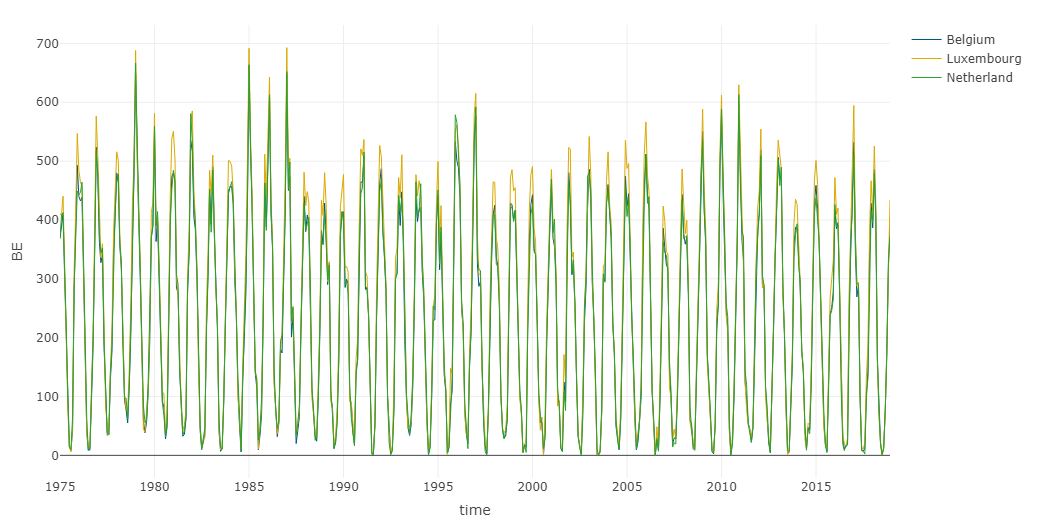
\includegraphics[width=\textwidth]{images/raw_data.jpeg}

There is an important technique for all types of time series data called decomposition. It seeks the construct of the data from an observations. Usually time series decomposed into:
\begin{itemize}
    \item T$_t$, the trend component at time t which is refers to a long term progression.
    \item C$_t$ the cyclical component at time t which reflects repeated but non-periodic fluctuations
    \item S$_t$ the seasonal component at time t, reflecting seasonality (seasonal variation).
    \item I$_t$the irregular component (or "noise") at time t, which describes random, irregular influences. 
\end{itemize}
For the forecasting I use the auto.arima function for the all column in the dataset, and after I select the common order for the 
After the decomposition we can see the trend in our data set.\newline    
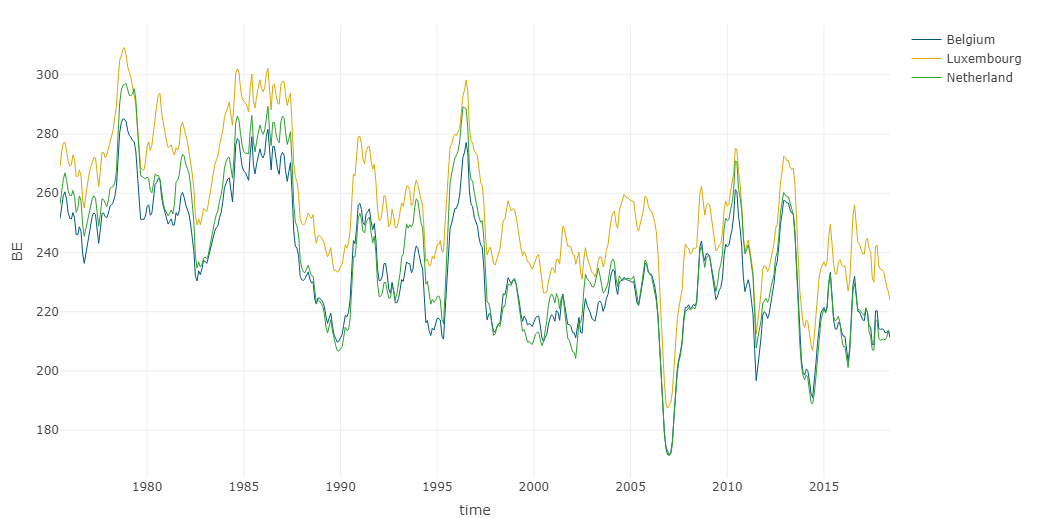
\includegraphics[width=\textwidth]{images/trend_data.jpeg}

\section*{Forecasting with VARMA model}

Vector autoregressive moving-average (VARMA) processes are suitable models for producing linear forecasts of sets of time series variables. A vector sequence y(t) of n elements is said to follow an n-variate ARMA process of orders p and q if it satisfies the equation: 
\[
A_{0}y(t) + A_{1}y(t-1) + .. + A_{p}y(t-p) =
    M_{0}\epsilon(t) + M_{1}\epsilon(t-1)+ .. + M_{p}\epsilon(t-p)
\]
where $A_{0}$, $A_{1}$, ... ,$A_{p}$, $M_{0}\epsilon$(t), $M_{1}\epsilon$(t-1), $M_{q}\epsilon$(t-q) are matrices of order n × n and $\epsilon$(t) is a disturbance vector of n elements determined by serially-uncorrelated white noise processes that may have some contemporaneous correlation.
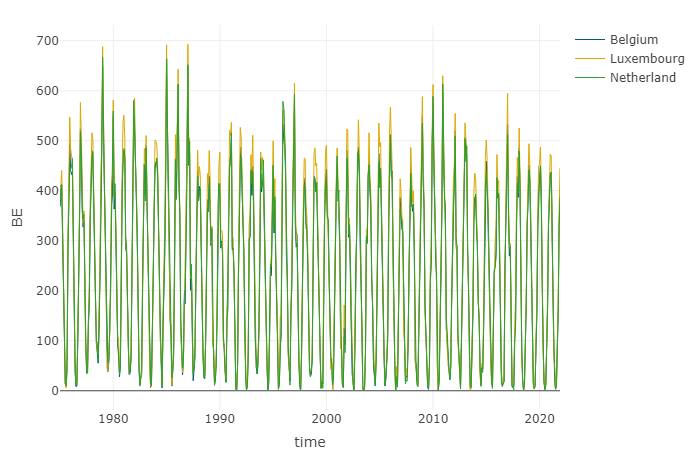
\includegraphics[width=\textwidth]{images/pred_data.jpeg}












\end{document}
